\section{Stratified Error Breakdown, Modal Profiles, and Tuning-Induced Regressions}
\label{app-stratified}

This chapter provides comprehensive error breakdowns across all evaluated decision-makers. We examine performance across urban dimensions, present pairwise decision concordance, and identify sub-populations where prompt engineering degrades accuracy.

\subsection{Dimension-Wise Weighted Error}

We compute the mean stratum $L_1$ error weighted by the population size of covered strata. Five dimensions enter the composite score: distance band, trip purpose, age bracket, occupation category, and gender. Two additional dimensions, residential ring and housing type, enter neither the composite loss nor the calibration cycle.

\begin{table*}[tp]
  \caption{Weighted $L_1$ error (\%) across urban dimensions and decision-makers.}
  \label{tab-dimensions-full}
  \begin{tabular}{lrrrrrrr}
    \toprule
    Decision-maker & Distance & Purpose & Age & Occupation & Gender & Ring & Housing \\
    \midrule
    \texttt{gemini-3.5}, minimal    & 24.1 & 27.9 & 30.6 & 25.3 & 23.9 & 25.7 & 30.5 \\
    \texttt{gemini-3.5}, expert     & \textbf{14.2} & 21.4 & 22.1 & 18.5 & 13.6 & 19.6 & 23.6 \\
    \texttt{gemini-3.1}, minimal    & 38.0 & 37.8 & 43.9 & 39.2 & 39.4 & 40.5 & 43.1 \\
    \texttt{gemini-3.1}, expert     & 30.2 & 30.8 & 35.8 & 31.2 & 30.7 & 33.0 & 37.4 \\
    \texttt{mistral-large}, minimal & 51.9 & 39.3 & 46.8 & 43.8 & 44.5 & 47.6 & 51.0 \\
    \texttt{mistral-large}, expert  & 33.7 & 27.9 & 30.4 & 28.6 & 25.3 & 29.6 & 33.0 \\
    \midrule
    Gradient boosting (LightGBM)    & 17.8 & \textbf{13.6} & 18.2 & 15.7 & 8.5 & 11.5 & 16.6 \\
    Random forest                   & 16.8 & 18.1 & \textbf{16.8} & \textbf{12.9} & \textbf{5.3} & \textbf{9.5} & \textbf{15.9} \\
    Kernel logistic regression     & 18.1 & 14.2 & 18.9 & 15.1 & 8.1 & 11.8 & 17.0 \\
    Multinomial logit               & 19.5 & 16.4 & 21.2 & 17.8 & 10.4 & 13.2 & 19.4 \\
    \bottomrule
  \end{tabular}
\end{table*}

Table~\ref{tab-dimensions-full} details the weighted $L_1$ errors across all deciders. Distance is the only dimension where an LLM agent achieves the lowest error across all benchmarked methods.



\subsection{Global Modal Share Distributions}

\begin{table*}[tp]
  \caption{Global modal split percentages across models against the survey.}
  \label{tab-shares-full}
  \begin{tabular}{lrrrr}
    \toprule
    Model & Car (\%) & Walking (\%) & Transit (\%) & Cycling (\%) \\
    \midrule
    Cerema EMC\textsuperscript{2} 2023 survey & 56.7 & 26.8 & 12.4 & 4.1 \\
    \midrule
    Minimal prompt, \texttt{gemini-3.5} & 47.4 & 24.0 & 20.9 & 7.6 \\
    Expert prompt, \texttt{gemini-3.5}  & 52.3 & 24.2 & 16.6 & 6.8 \\
    Minimal prompt, \texttt{gemini-3.1} & 44.1 & 19.5 & 28.8 & 7.7 \\
    Expert prompt, \texttt{gemini-3.1}  & 46.2 & 21.7 & 24.8 & 7.4 \\
    Minimal prompt, \texttt{mistral-large} & 36.7 & 24.4 & 30.6 & 8.2 \\
    Expert prompt, \texttt{mistral-large}  & 43.4 & 29.3 & 19.2 & 8.1 \\
    \midrule
    Gradient boosting (LightGBM)        & 52.8 & 29.1 & 14.8 & 3.3 \\
    Random forest                       & 56.2 & 27.6 & 14.2 & 2.0 \\
    Kernel logistic regression          & 54.4 & 28.9 & 13.6 & 3.0 \\
    Multinomial logit                   & 53.3 & 27.2 & 16.4 & 3.0 \\
    \bottomrule
  \end{tabular}
\end{table*}

Table~\ref{tab-shares-full} compares predicted modal shares against the empirical Cerema survey ground truth. Every decider underestimates car usage because vehicle chaining constraints enforce strict feasibility checks.

Language models overestimate cycling by a factor of two across all weighted strata. Conversely, supervised tabular models systematically underestimate cycling shares.



\subsection{Visualizations of Multi-Dimensional Error Profiles}

\begin{figure*}[tp]
  \centering
  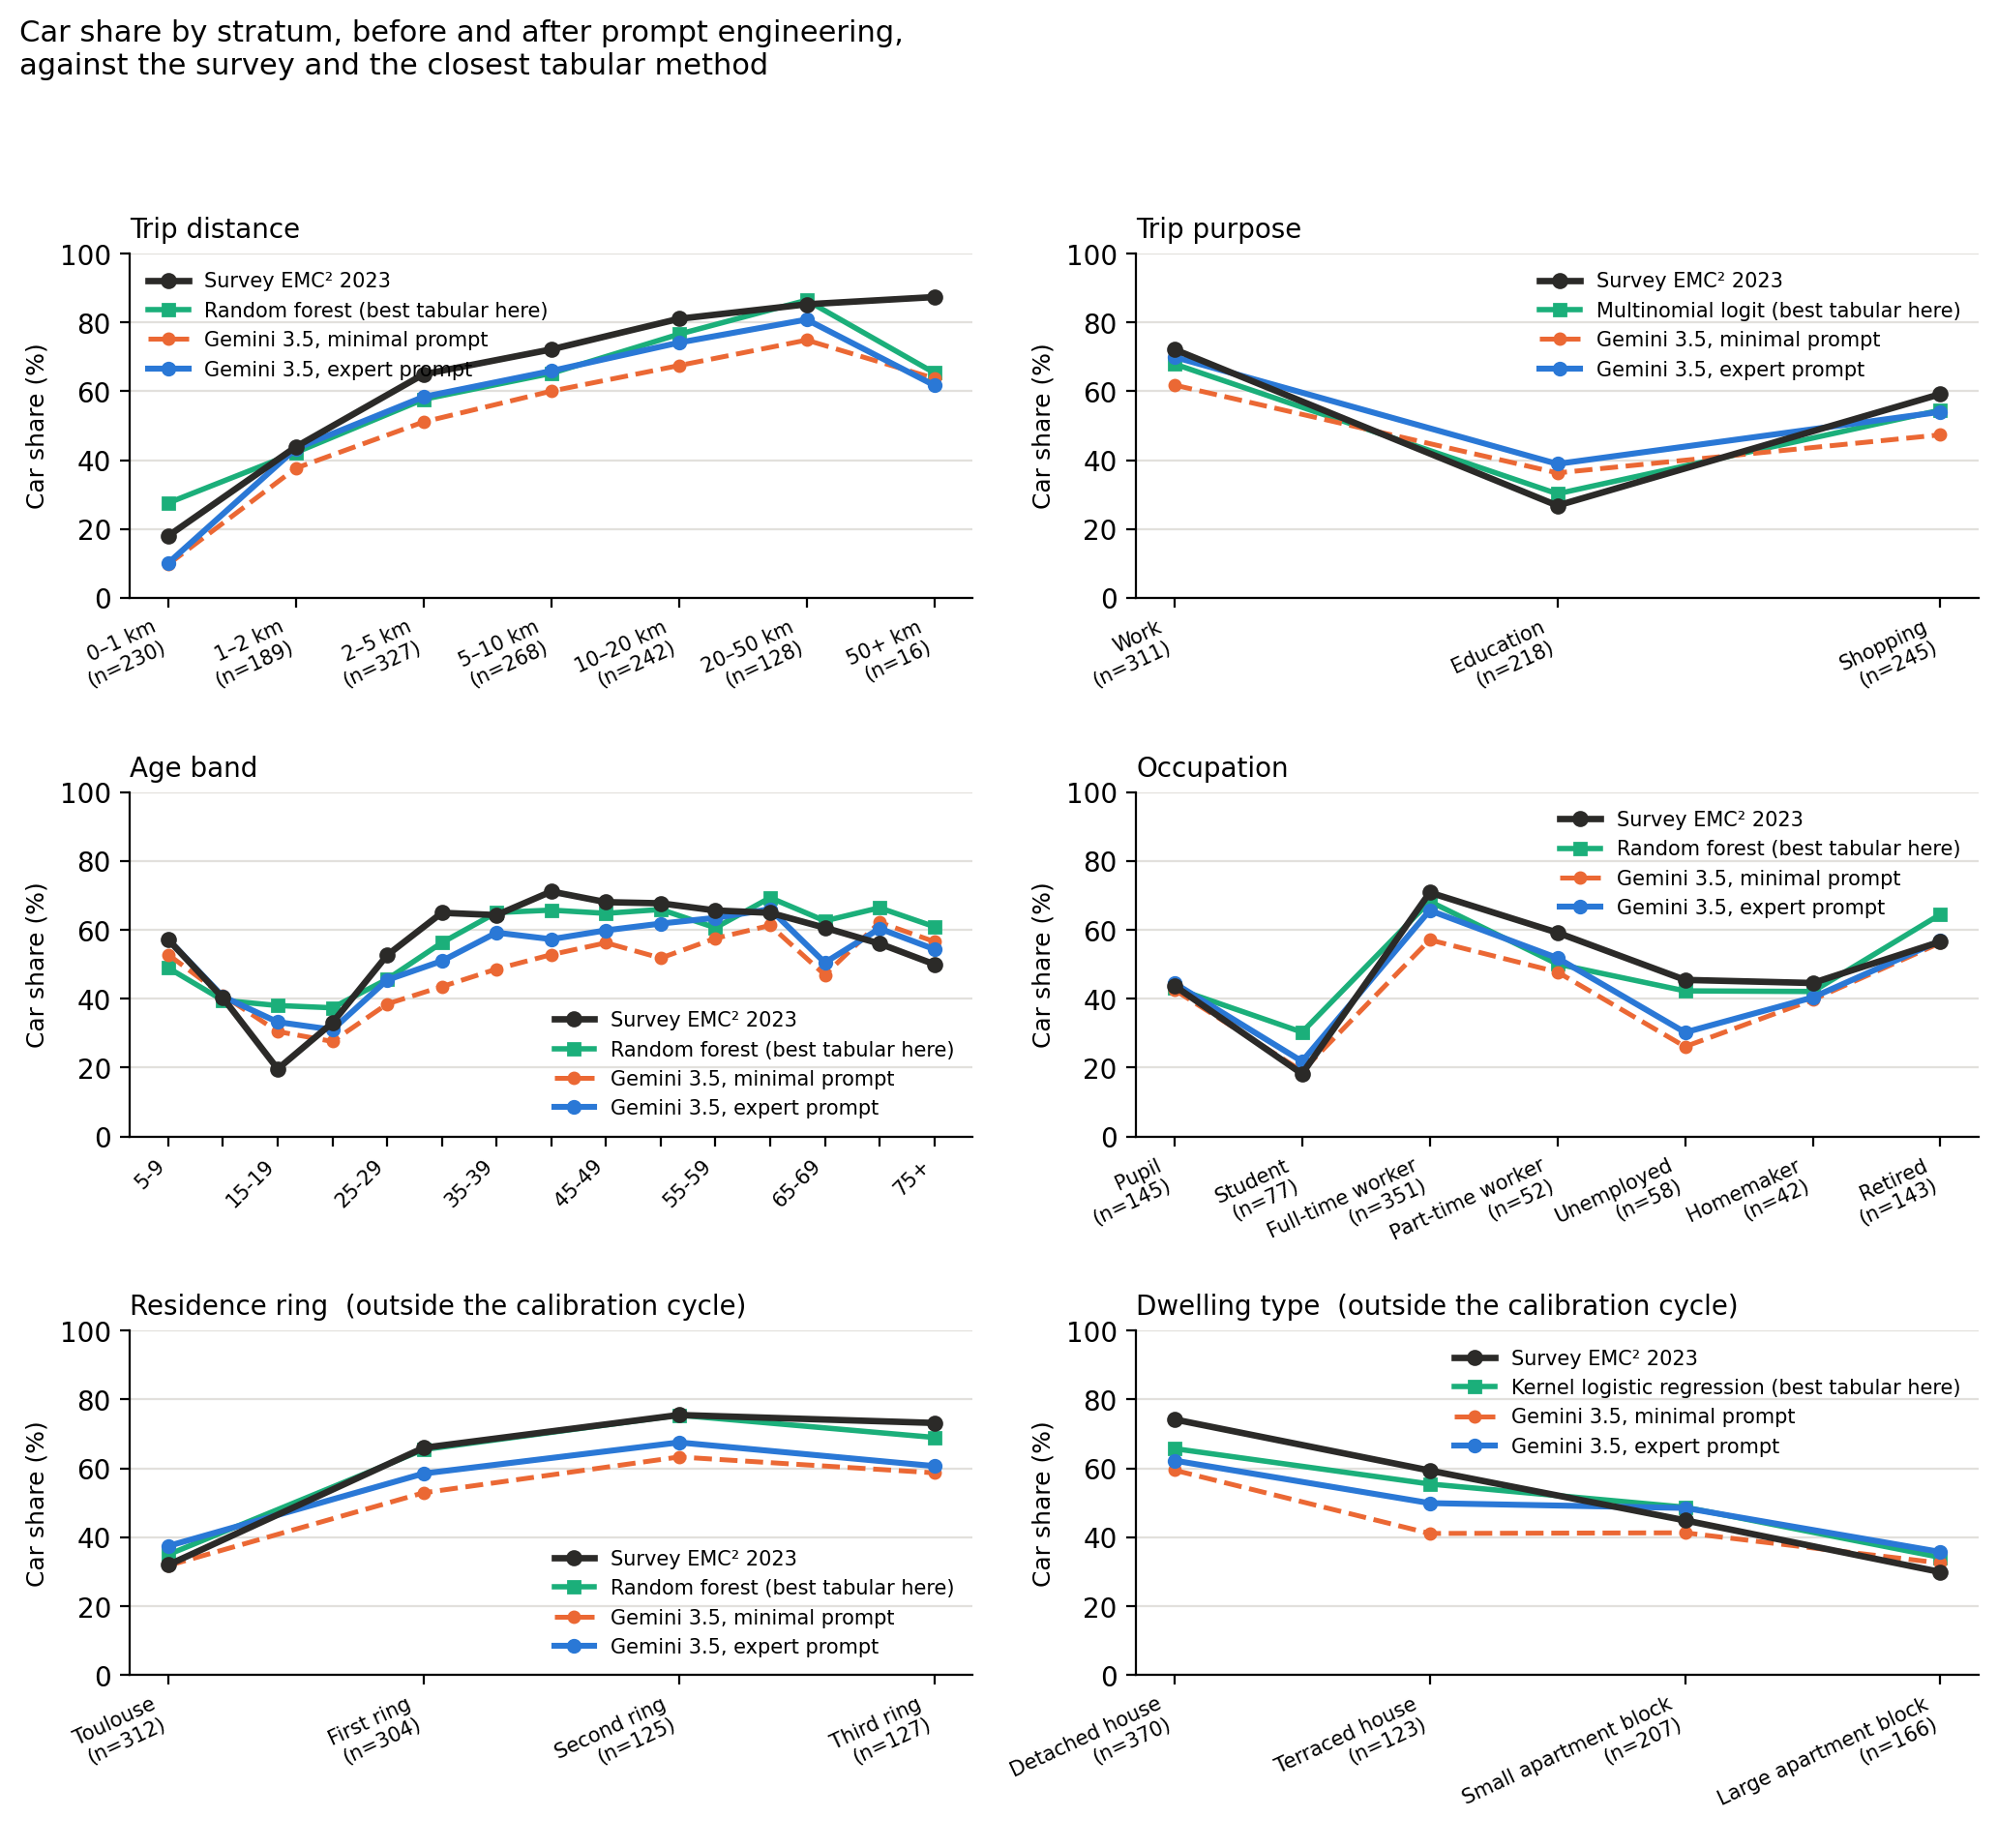
\includegraphics[width=\textwidth]{images/ch99_dimensions_voiture.png}
  \caption{Car share by stratum across six dimensions, minimal vs expert prompt against survey and tabular reference.}
  \label{fig-dim-voiture}
\end{figure*}

\begin{figure*}[tp]
  \centering
  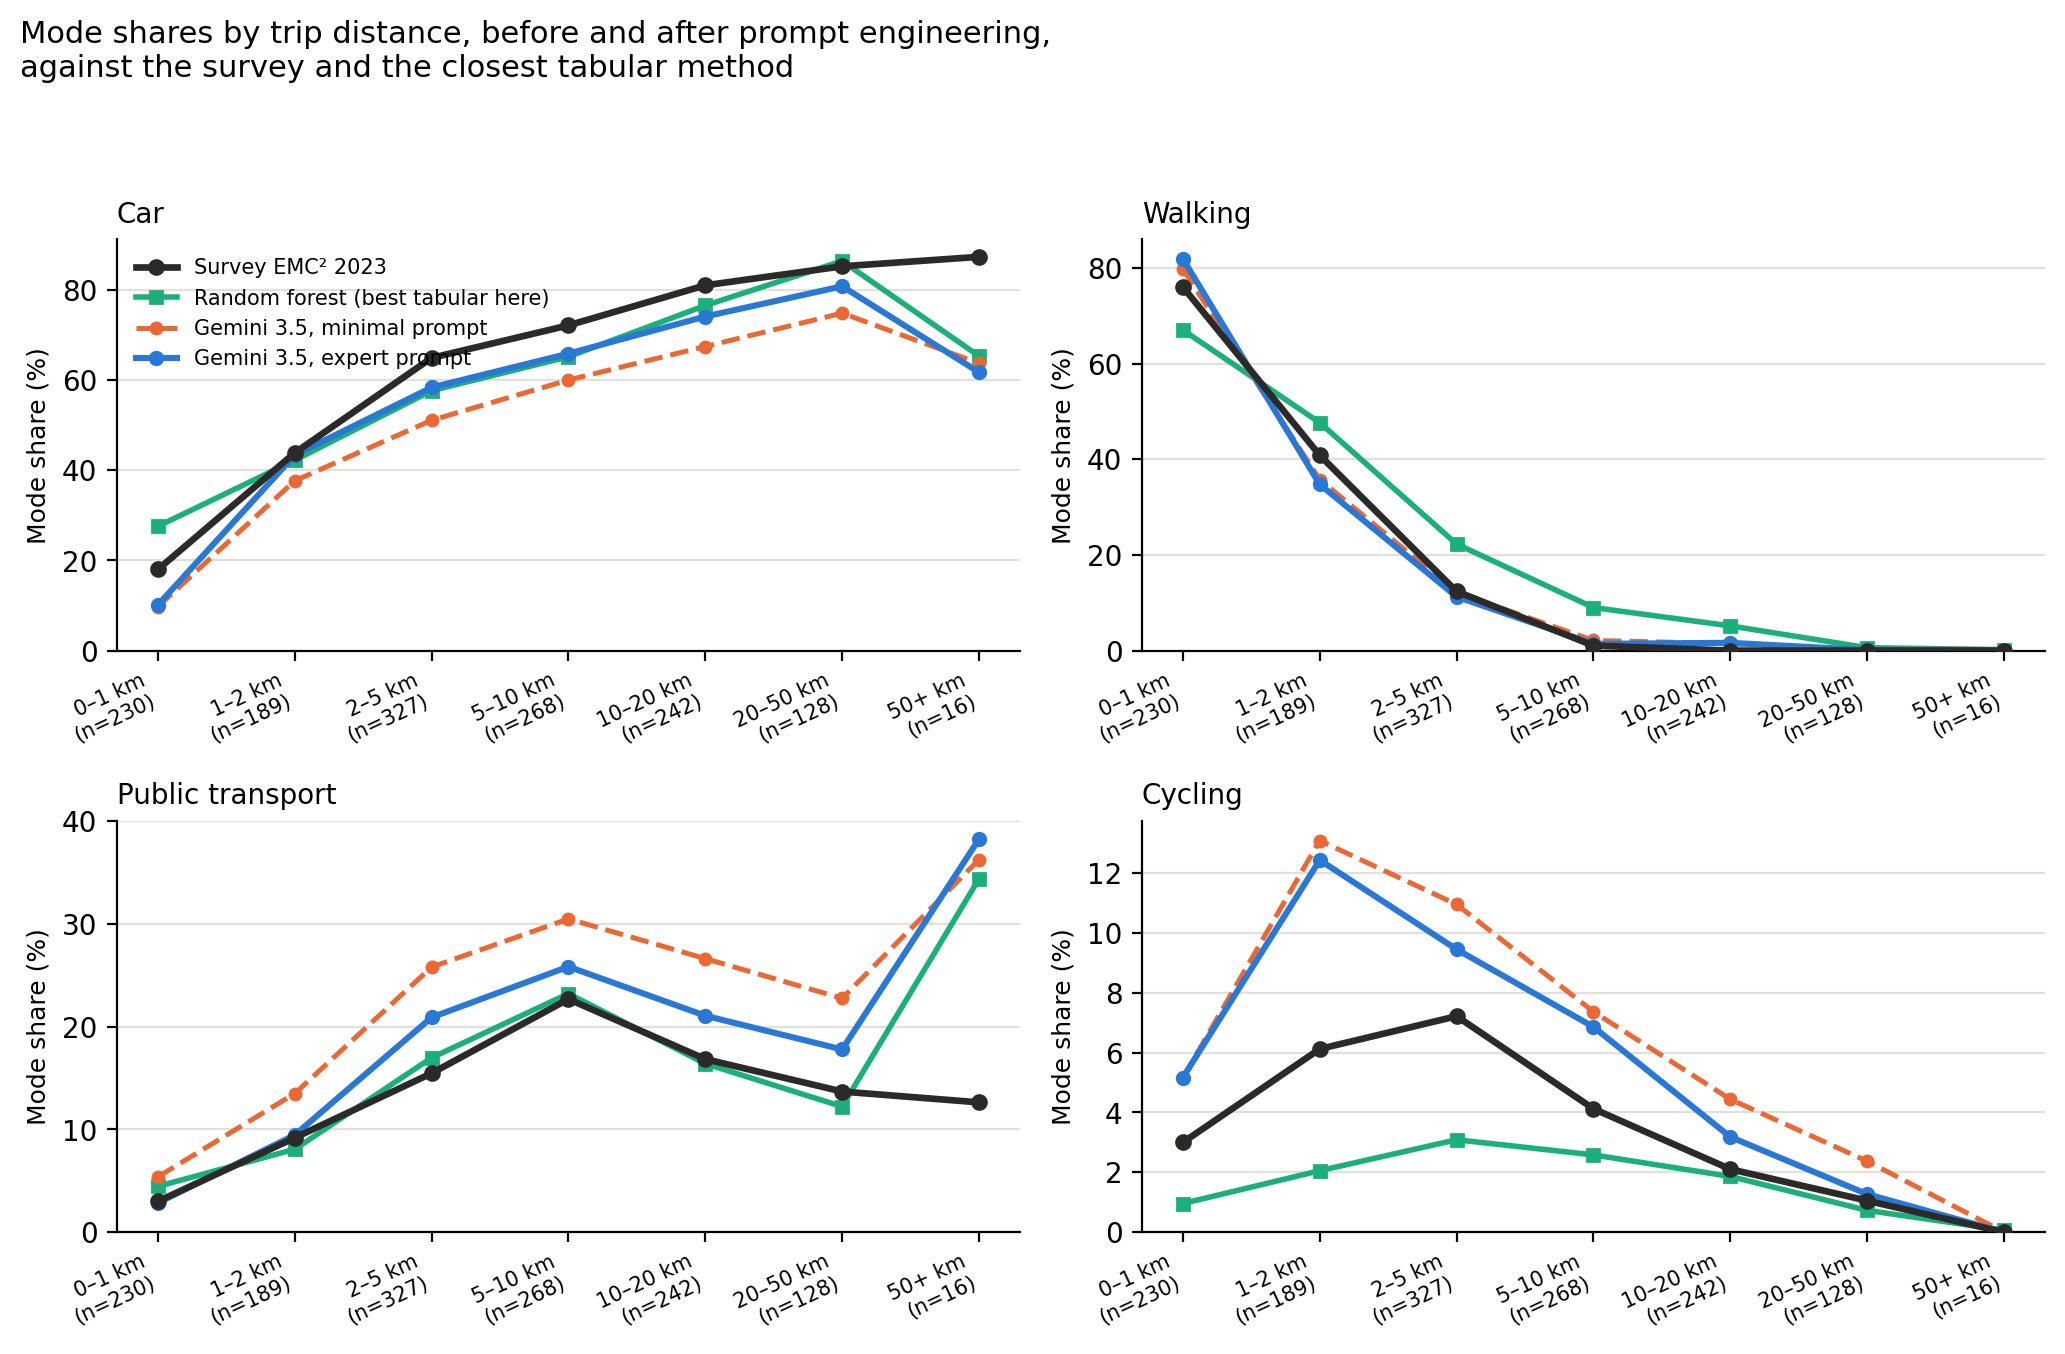
\includegraphics[width=\textwidth]{images/ch99_modes_distance.png}
  \caption{Four transport modes broken down by distance band.}
  \label{fig-modes-dist}
\end{figure*}

\begin{figure*}[tp]
  \centering
  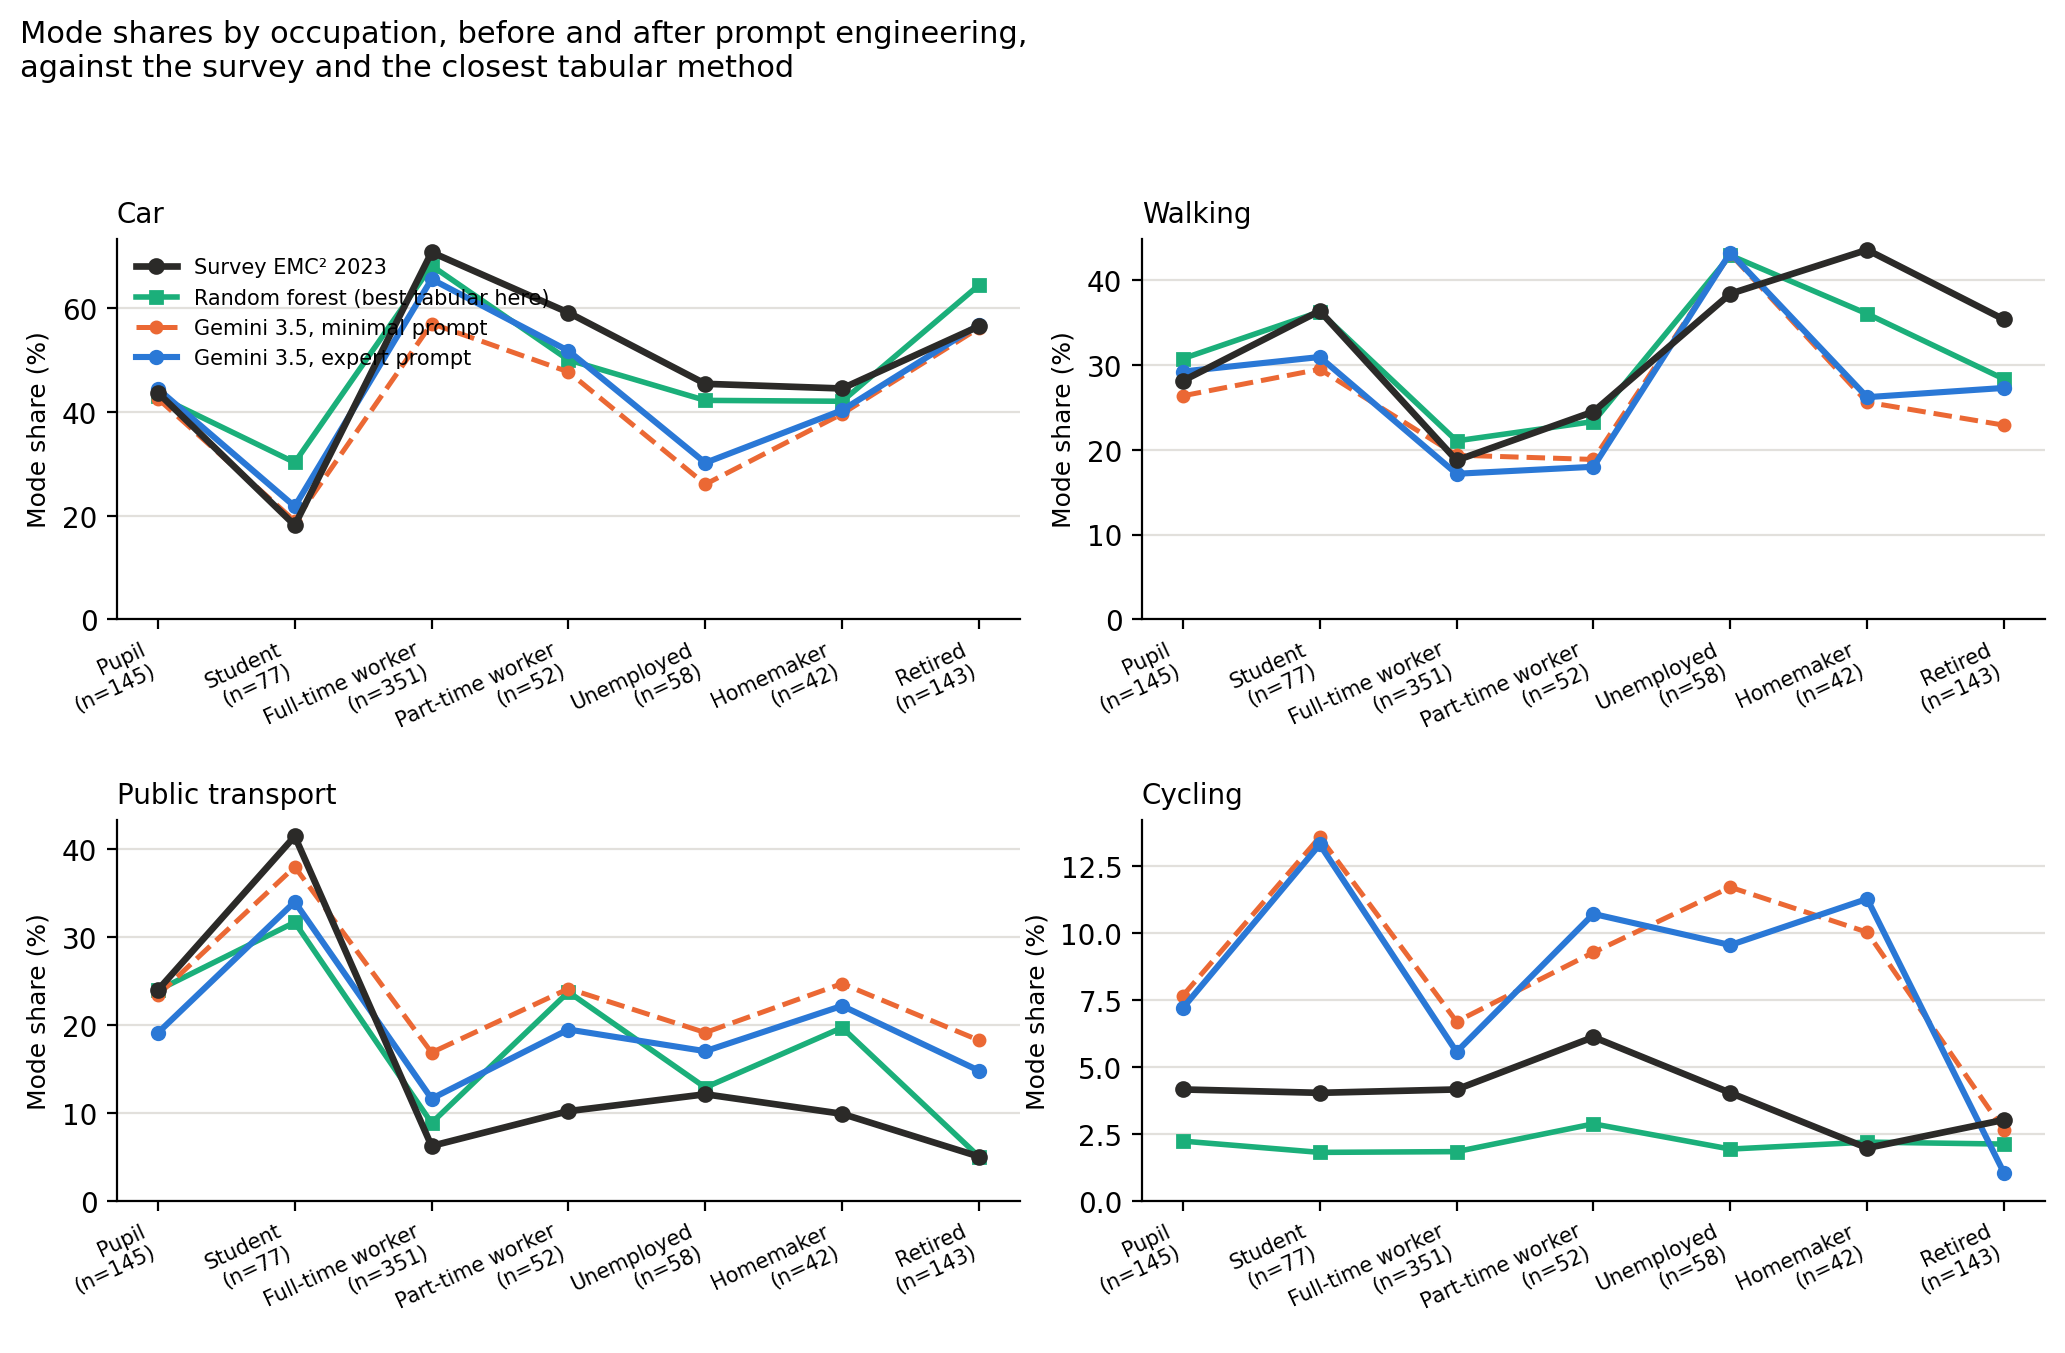
\includegraphics[width=\textwidth]{images/ch99_modes_occupation.png}
  \caption{Four transport modes across eight occupation categories.}
  \label{fig-modes-occ}
\end{figure*}

\begin{figure*}[tp]
  \centering
  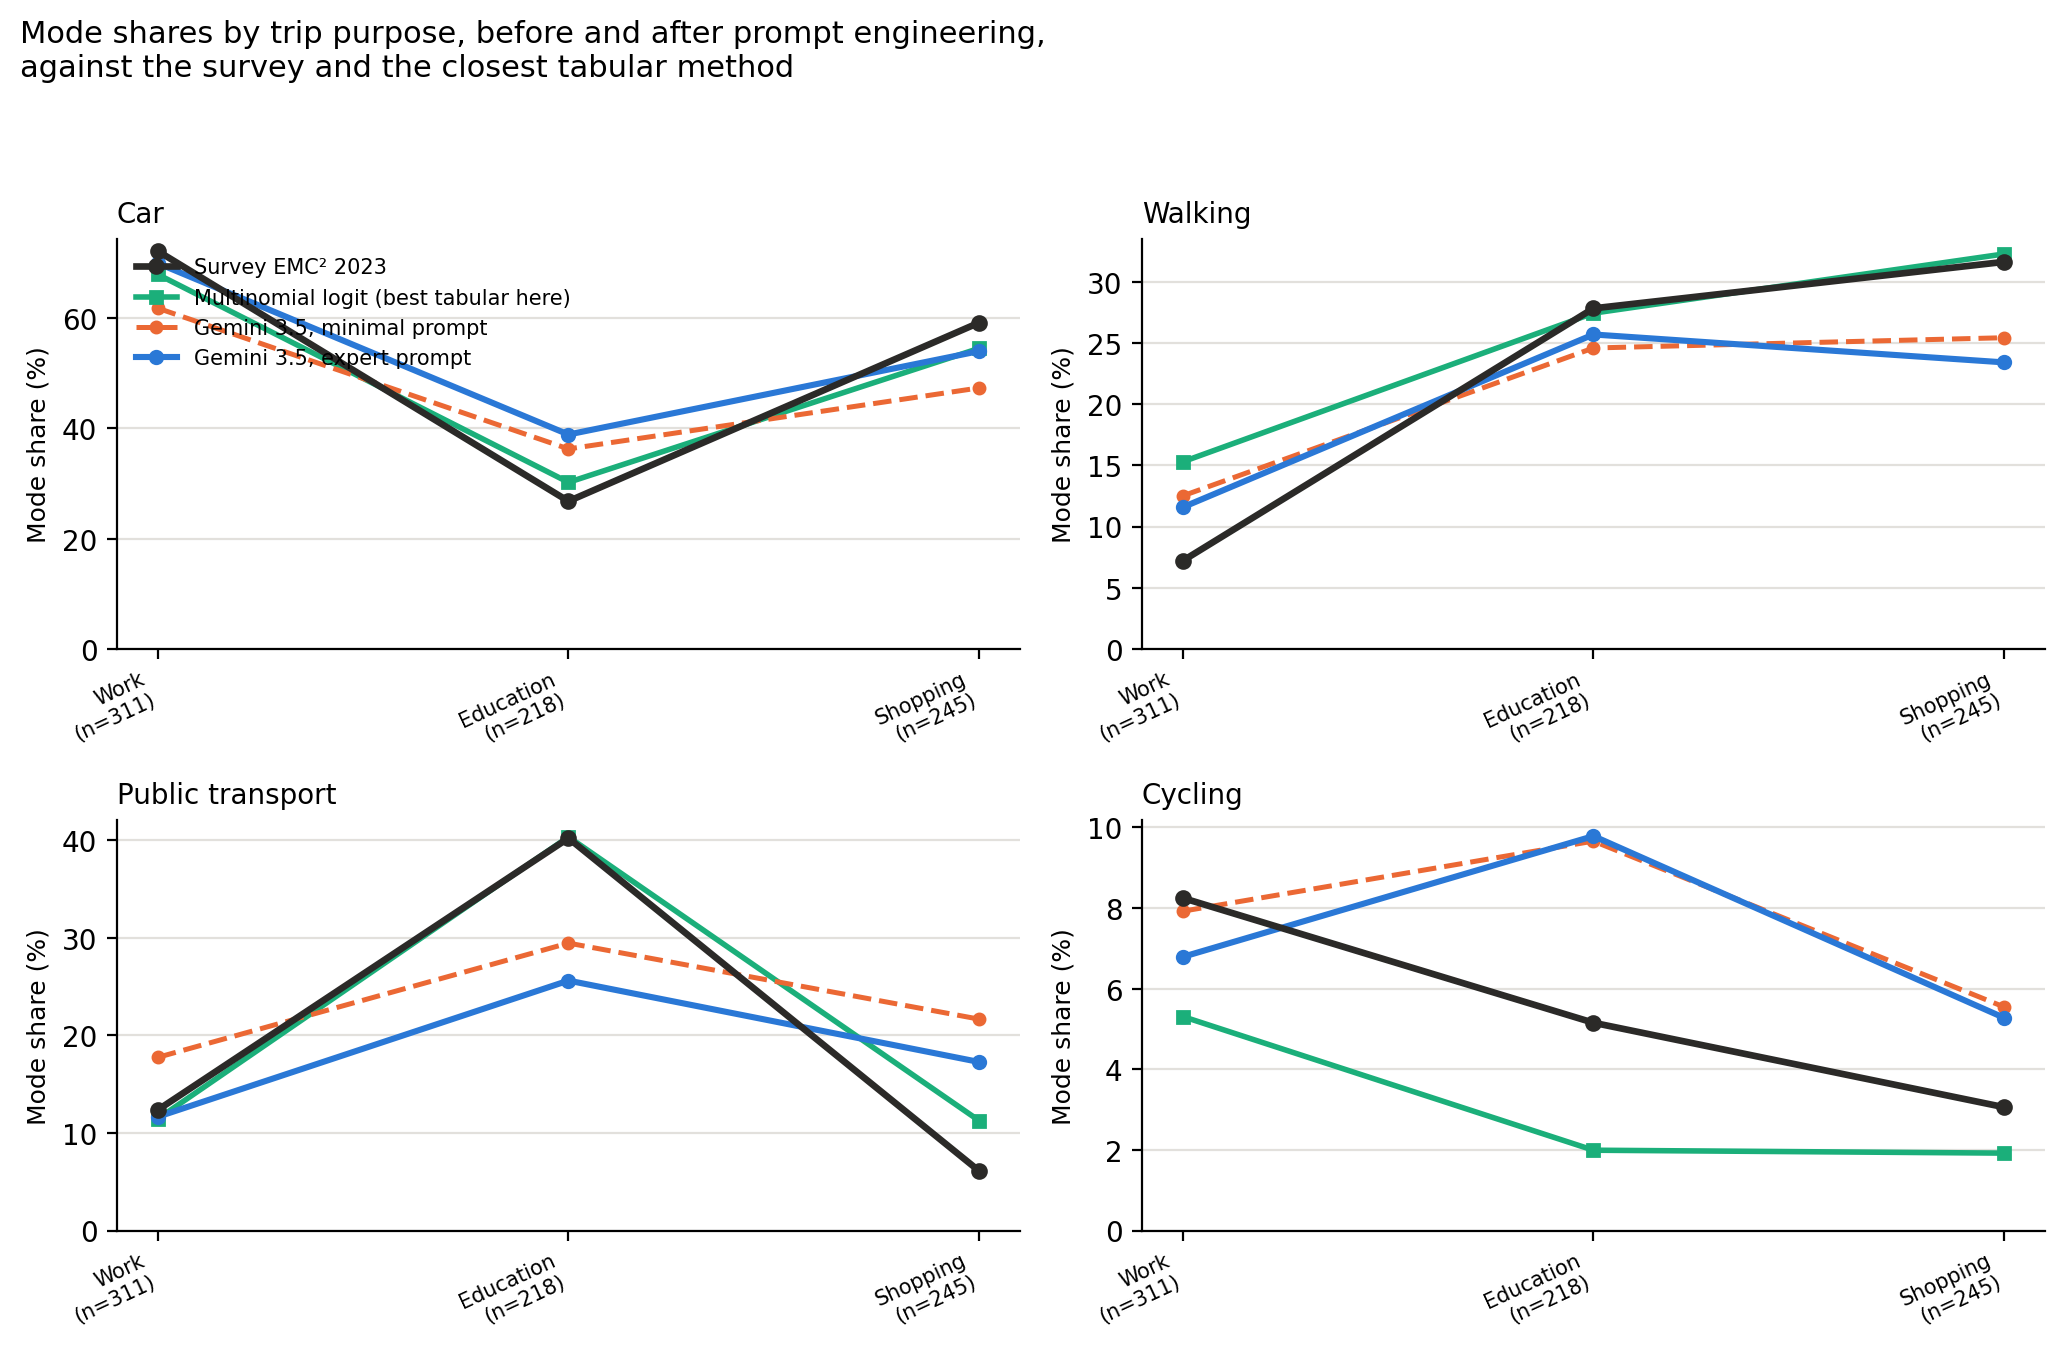
\includegraphics[width=\textwidth]{images/ch99_modes_motif.png}
  \caption{Four transport modes across six trip purposes.}
  \label{fig-modes-motif}
\end{figure*}

We provide four multi-panel visual figures examining stratified modal behavior.

Figure~\ref{fig-dim-voiture} displays car shares across six dimensions. On the first four dimensions, the expert prompt sits substantially closer to the target than the minimal baseline. On residential ring and housing type, both LLM series remain distant from empirical targets.

Figure~\ref{fig-modes-dist} breaks down the four transport modes by distance band. Car and walking predictions closely track ground truth beyond one kilometer. Public transit displays persistent overestimation between two and twenty kilometers.

Figure~\ref{fig-modes-occ} examines modal distributions across eight occupation categories. School-age categories exhibit the highest cycling shares, reaching 8.2\% and 13.3\% under the expert prompt versus 4.2\% and 4.0\% in the survey.

Figure~\ref{fig-modes-motif} plots the four modes across six trip purposes. Educational trips produce the largest divergence following prompt engineering, shifting heavily toward private vehicles.


\subsection{Strata Degraded by Expert Prompt Tuning}

\begin{table}[tbp]
  \caption{Stratum $L_1$ errors (\%) degraded after expert prompt engineering.}
  \label{tab-degraded-full}
  \small
  \begin{tabularx}{\columnwidth}{@{}Lrrr@{}}
    \toprule
    Stratum and model & Minimal & Expert & Net gap \\
    \midrule
    Education, \texttt{gemini-3.5} ($n = 218$)    & 28.0 & 33.5 & $+5.5$ pt \\
    Education, \texttt{gemini-3.1} ($n = 218$)    & 20.0 & 21.2 & $+1.2$ pt \\
    Education, \texttt{mistral-large} ($n = 218$) &  8.7 & 22.3 & $+13.6$ pt \\
    15--19 years, \texttt{gemini-3.5} ($n = 61$)    & 53.4 & 58.3 & $+4.9$ pt \\
    15--19 years, \texttt{gemini-3.1} ($n = 61$)    & 49.2 & 47.9 & $-1.3$ pt \\
    15--19 years, \texttt{mistral-large} ($n = 61$) & 34.1 & 44.9 & $+10.8$ pt \\
    Trips $> 50$ km, \texttt{gemini-3.5} ($n = 19$) & 42.1 & 51.4 & $+9.3$ pt \\
    \bottomrule
  \end{tabularx}
\end{table}

Prompt engineering does not improve performance across all demographic segments. Table~\ref{tab-degraded-full} identifies sub-populations where the expert prompt degraded accuracy relative to the uncalibrated baseline.



The degradation on educational trips appears across all three language models. The prompt emphasizes travel speed and vehicle utility, inadvertently prompting students who lack private vehicles to select cars. Trips exceeding 50 kilometers similarly resist calibration across all deciders.

\subsection{Decision-by-Decision Concordance Between Deciders}

\begin{table*}[tp]
  \caption{Pairwise concordance across common trips with multiple available alternatives.}
  \label{tab-concordance}
  \begin{tabular}{lrrr}
    \toprule
    Model comparison pair & Concordance mode (\%) & Drawn mode (\%) & Median $L_1$ gap \\
    \midrule
    Gradient boosting / Kernel regression & 91.6 & 90.5 & 8.3 \\
    Gradient boosting / Random forest     & 89.0 & 88.3 & 11.3 \\
    \midrule
    Expert \texttt{gemini-3.5} / Gradient boosting & 69.7 & 61.4 & 39.0 \\
    Expert \texttt{gemini-3.5} / Random forest     & 71.4 & 60.4 & 42.6 \\
    Expert \texttt{gemini-3.5} / Expert \texttt{gemini-3.1}    & 79.6 & 72.8 & 40.0 \\
    Expert \texttt{gemini-3.1} / Expert \texttt{mistral-large} & 72.6 & 70.6 & 40.0 \\
    \bottomrule
  \end{tabular}
\end{table*}

We evaluate agreement across 2{,}374 to 2{,}479 trips where at least two alternatives were available. Table~\ref{tab-concordance} summarizes concordance between model pairs.

Tabular models display high mutual agreement, exceeding 88\,\% on drawn choices. Conversely, LLMs diverge sharply from tabular references, exhibiting median $L_1$ distances near 40 percentage points.



\subsection{Non-Convex Optimization and Prompt Trajectory}

\begin{table*}[tp]
  \caption{Evaluation metrics across prompt engineering iterations on \texttt{gemini-3.5-flash-lite}.}
  \label{tab-prompt-traj}
  \begin{tabular}{llrrr}
    \toprule
    Prompt variant & Engineering status & Composite & Excl.\ s.c. & Macro $L_1$ (\%) \\
    \midrule
    \texttt{prompt\_minimal\_02} & Baseline without engineering   & 7.02 & 10.39 & 24.08 \\
    \texttt{prompt\_expert\_05}  & General cognitive ablation     & 4.86 &  6.86 & 13.85 \\
    \texttt{prompt\_expert\_06}  & Tuned on cohort residuals      & 5.33 &  7.24 & 15.39 \\
    \texttt{prompt\_expert\_08}  & Heavily tuned on residuals     & 6.58 & 10.32 & 21.74 \\
    \bottomrule
  \end{tabular}
\end{table*}

We tracked iterative prompt modifications evaluated on \texttt{gemini-3.5-flash-lite}. Table~\ref{tab-prompt-traj} documents the resulting composite scores.

Variants tailored directly to sample residuals (\texttt{prompt\_expert\_06} and \texttt{08}) degraded aggregate performance. In contrast, \texttt{prompt\_expert\_05} retained general cognitive principles, achieving superior generalization. This pattern highlights the non-convex optimization surface characteristic of natural language prompts.


